\chapter{RUMIS - Nonmonotonic Rule Mining System}\label{chap:system}

RUMIS stands for Nonmonotonic Rule Mining System which is the main tool developed from the current work. In this chapter, our system are described in details with the following organization. Firstly, an overview of the system is mentioned. Secondly, the main method with a novel concept of Partial Materialization is discussed. Finally, we talk about the implementation of components in the system.

\section{System Overview}

There are five components in the system as indicated in Figure~\ref{system_overview}. The RUMIS receipts an input as a set of mined positive Horn rules and a knowledge graph. The corresponding output is a set of nonmonotonic rules derived from given Horn rules by adding negated atoms. The five components are described in details in the rest of this chapter.

\begin{figure}[ht]
\centering
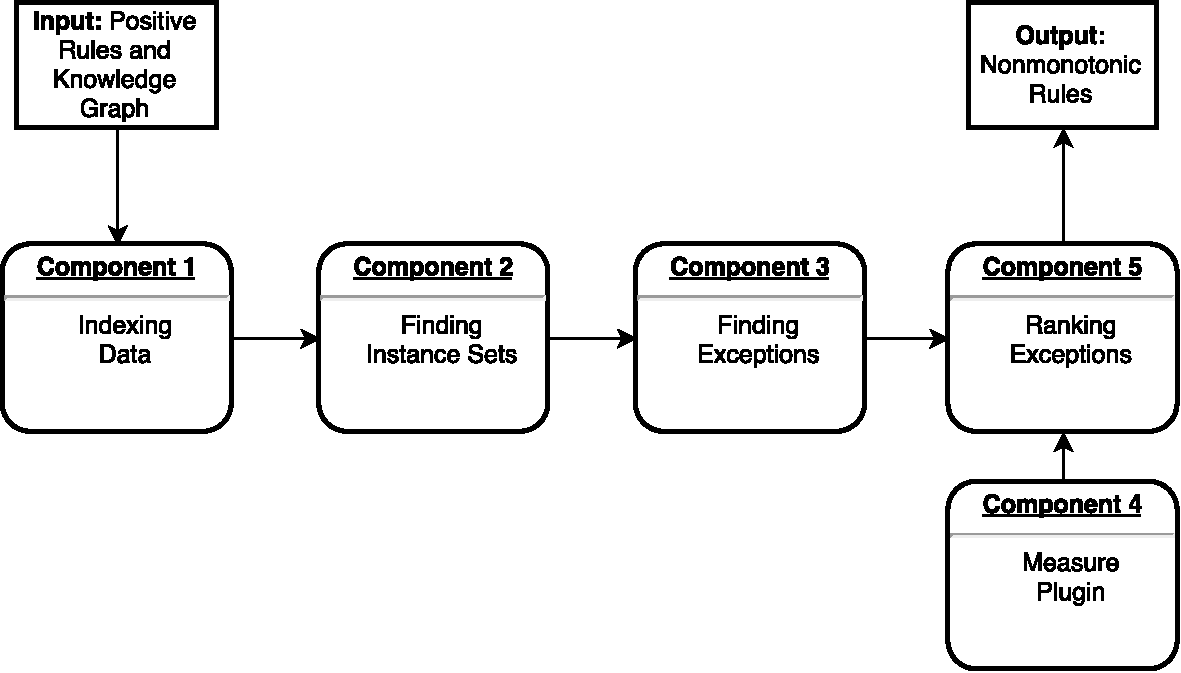
\includegraphics[width=0.75\textwidth]{figures/system_overview}
\caption{Components of the RUMIS}
\label{system_overview}
\end{figure}

\section{Implementation}

\subsection{Data Indexing}

\begin{figure}[ht]
\centering
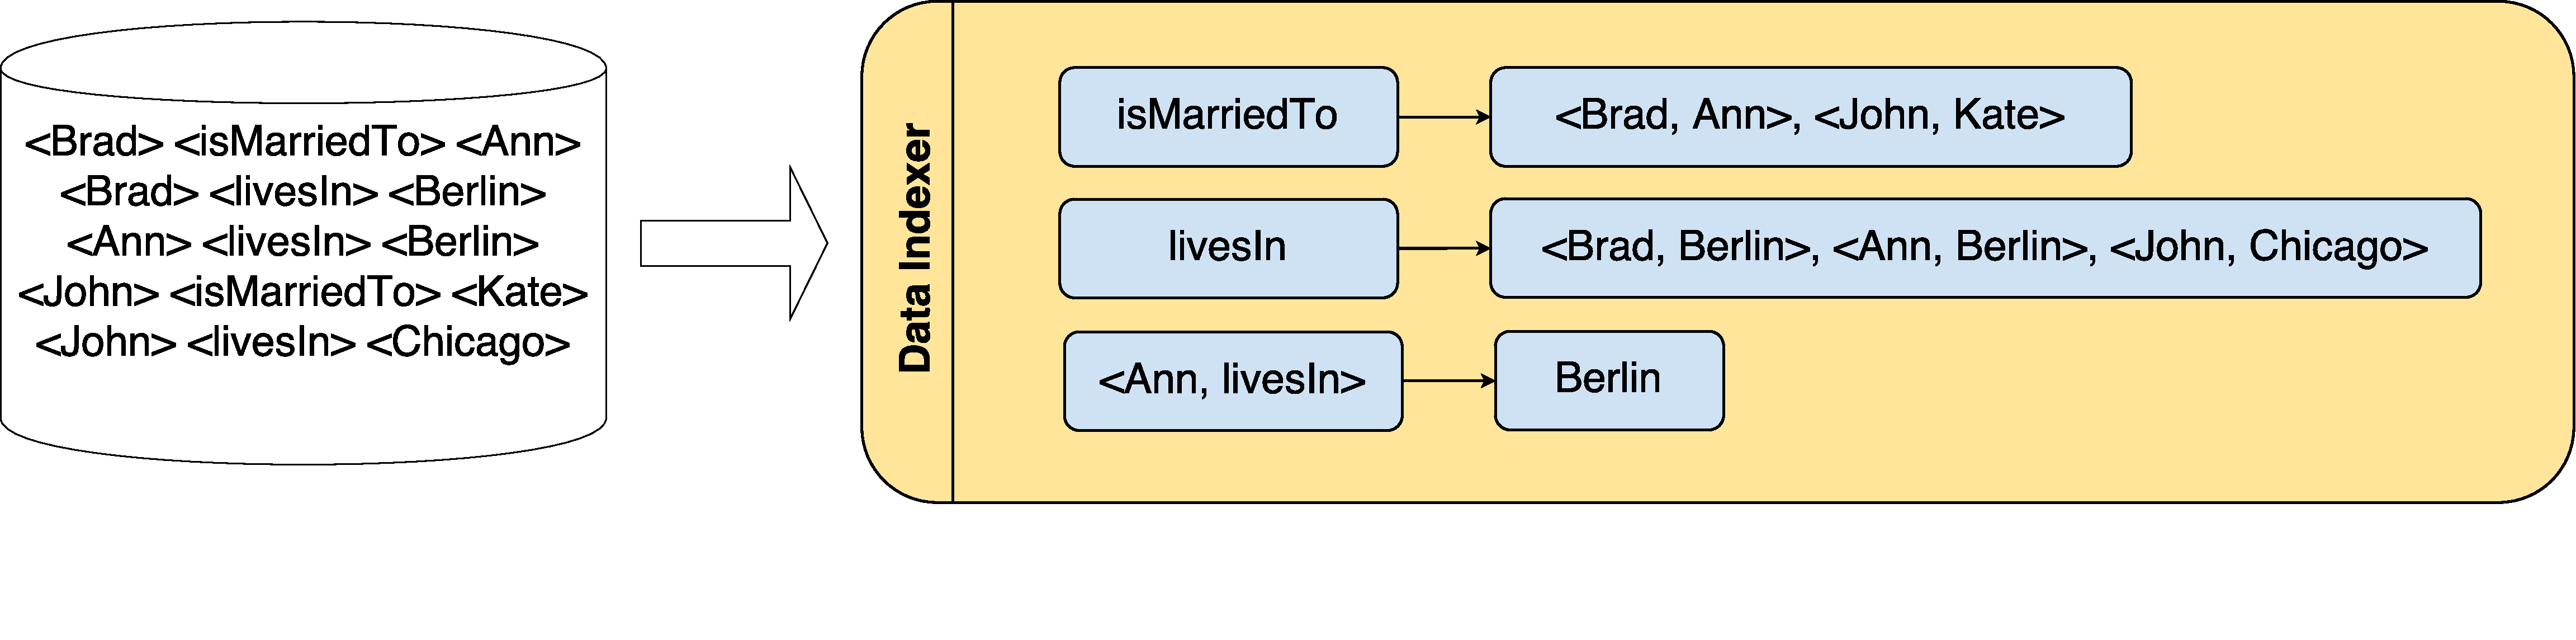
\includegraphics[width=1.0\textwidth]{figures/data_indexing}
\caption{RUMIS Data Indexer}
\label{system_overview}
\end{figure}

\subsection{Positive Rule Mining}

Pseudocode and explanation.

\IncMargin{1.5em}
\begin{algorithm}[H]
\DontPrintSemicolon
\SetAlgoLined
\SetKwInOut{Input}{Input}\SetKwInOut{Output}{Output}
\Input{KG $\cG$}
\Output{Set of positive rules with the form \textit{h(X, Z) $\leftarrow$ p(X, Y), q(Y, Z)}}
\BlankLine
$absSupp \leftarrow \{\}$\\
\BlankLine
\ForEach{Triple $YqZ$ in $\cG$} {
    \BlankLine
	$pXSet \leftarrow getPredicateSubjectSet(\cG, Y)$\\
	\ForEach{Pair $pX$ in $pXSet$} {
		$hSet \leftarrow getPredicateSet(\cG, X, Z)$\\
		$absSupp[hpq]++$\\
%        \uIf{If condition}{
%            instruction
%        }
%        \uElseIf{ElseIf condition}{
%            instruction
%        }
%        \uElse{
%            instruction
%        }
	}
}
\BlankLine
Sort $hpq$ according to deacreasing order of $absSupp[hpq]$\\
\Return $absSupp$\\
\caption{Positive Rule Mining}
\end{algorithm}
\DecMargin{1.5em}

%\begin{algorithm}[H]
%\DontPrintSemicolon
%\SetAlgoLined
%\KwResult{Write here the result}
%\SetKwInOut{Input}{Input}\SetKwInOut{Output}{Output}
%\Input{Write here the input}
%\Output{Write here the output}
%\BlankLine
% 
%\While{While condition}{
%    instructions\;
%    \eIf{condition}{
%        instructions1\;
%        instructions2\;
%    }{
%        instructions3\;
%    }
%}
% 
%\caption{While loop with If/Else condition}
%\end{algorithm}

\subsection{Normal and Abnormal Set Mining}

Pseudocode and explanation.

\IncMargin{1.5em}
\begin{algorithm}[H]
\DontPrintSemicolon
\SetAlgoLined
\SetKwInOut{Input}{Input}\SetKwInOut{Output}{Output}
\Input{KG $\cG$, $h$, $p$, $q$}
\Output{Normal and abnormal sets of the rule \textit{h(X, Z) $\leftarrow$ p(X, Y), q(Y, Z)}}
\BlankLine
$NS \leftarrow \{\}$\\
$ABS \leftarrow \{\}$\\
$YZSet \leftarrow getSubjectObjectSet(\cG, q)$\\
\BlankLine
\ForEach{Pair $YZ$ in $YZSet$} {
    \BlankLine
	$XSet \leftarrow getSubjectSet(\cG, p, Y)$\\
	\ForEach{$X$ in $XSet$} {
	\uIf{$XhZ$ is in $\cG$} {
		Add $XZ$ to $NS$\\
	}
	\uElse {
		Add $XZ$ to $ABS$\\
	}
%        \uElse{
%            instruction
%        }
	}
}
\BlankLine
\Return $NS$ and $ABS$\\
\caption{Normal and Abnormal Set Mining}
\end{algorithm}
\DecMargin{1.5em}

\subsection{Exception Witness Set Mining}

Pseudocode and explanation.

\IncMargin{1.5em}
\begin{algorithm}[H]
\DontPrintSemicolon
\SetAlgoLined
\SetKwInOut{Input}{Input}\SetKwInOut{Output}{Output}
\Input{KG $\cG$, $h$, $p$, $q$}
\Output{Exception witness Set of the rule \textit{h(X, Z) $\leftarrow$ p(X, Y), q(Y, Z)}}
\BlankLine
$NS \leftarrow getNormalSet(\cG, h, p, q)$\\
$ABS \leftarrow getAbnormalSet(\cG, h, p, q)$\\
$EWS+ \leftarrow \{\}$
$EWS- \leftarrow \{\}$
\BlankLine
\ForEach{Pair $XZ$ in $ABS$} {
	$pSet \leftarrow getPredicateSet(\cG, X, Z)$\\
	$EWS+$ $\leftarrow$ $EWS+$ $\cup$ $pSet$\\
}
\ForEach{Pair $XZ$ in $NS$} {
	$pSet \leftarrow getPredicateSet(\cG, X, Z)$\\
	$EWS-$ $\leftarrow$ $EWS-$ $\cup$ $pSet$\\
}
$EWS$ $\leftarrow$ $EWS+$ $\setminus$ $EWS-$\\
\Return $EWS$\\
\caption{Exception Witness Set Mining}
\end{algorithm}
\DecMargin{1.5em}

\subsection{Measure Plugin}

Just description text.

\subsection{Exception Ranking}

Should use at least one designed picture.

\begin{figure}[ht]
\centering
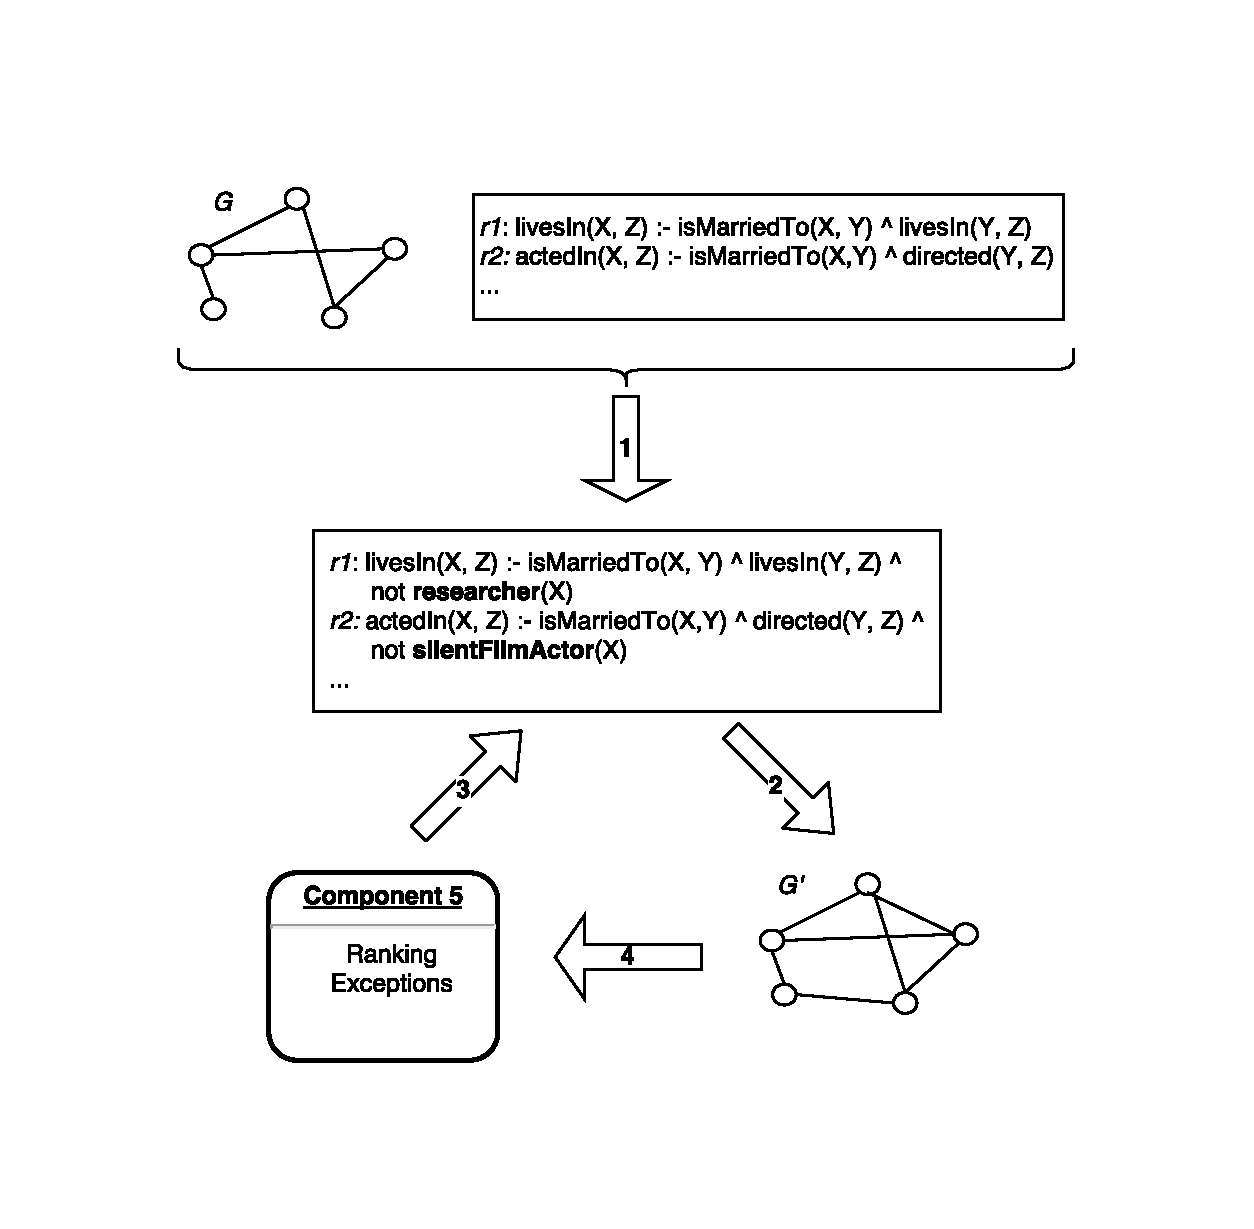
\includegraphics[width=1.0\textwidth]{figures/ranking}
\caption{Partial Materialization Ranking}
\label{pm_ranking}
\end{figure}

\textbf{OPM Ranking.} Describe...

\IncMargin{1.5em}
\begin{algorithm}[H]
\DontPrintSemicolon
\SetAlgoLined
\SetKwInOut{Input}{Input}\SetKwInOut{Output}{Output}
\Input{KG $\cG$, Set of positive rules $\cR_{H}$}
\Output{Set of best revisions $R_{NM}$ for the given positive rules}
\BlankLine
$\cG' \leftarrow \cG$\\
$R_{NM} \leftarrow \{\}$\\
\BlankLine
\ForEach{Rule $r$ in $R_H$} {
	Rank exceptions of $r$ based on $\cG'$, choose $r'$ as the best revision of $r$\\
	Add $r'$ to $R_{NM}$\\
	Predict new facts by applying all revisions of $r$ to $\cG$ then index these facts to $\cG'$\\
}
\Return $R_{NM}$\\
\caption{OPM Ranking}
\end{algorithm}
\DecMargin{1.5em}

%\section{Optimisation}
%
%I will talk about speeding up PM ranking in this section.

\section{Usage}

%\section{Discussion}
%\label{system:discuss}
%
%I will add RI lab part here.

%\subsection{INTRODUCTION}
%This report proposes a predicate abstraction algorithm for an RDF\footnote{\url{https://en.wikipedia.org/wiki/Resource_Description_Framework}} graph. More specifically, given an RDF file containing a set of subject-predicate-object triples \textit{<SPO>}, the algorithm focuses on \textbf{selecting types} for objects $O$ and uses these types for \textbf{abstracting} binary facts to unary ones.
%
%\begin{example}
%\label{ex1}
%Consider a fragment of an RDF graph given as a set of triples: \textit{<BillGates type person>, <BillGates type millionaire>, <Britney type singer>, <Britney type person>, <Melinda marriedTo BillGates>, <Kevin marriedTo Britney>, <Katy type singer>, <Katy type person>, <Brand marriedTo Katy>, <Kevin bornIn America>, \\<Brand bornIn America>}.
%\end{example}
%
%Every such triple \textit{<SPO>} can be represented as a binary fact \textit{P(S, O)} if \textit{P} is not \textit{type} and a unary fact \textit{O(S)} otherwise (e.g. \textit{<Kevin marriedTo Britney>, <BillGates type person>} can be seen as \textit{marriedTo(Kevin, Britney)} and \textit{person(BillGates)}, respectively). The goal of the algorithm is to select a type of \textit{Britney}, e.g., \textit{singer} among all of the types of this entity, and, construct a unary fact, e.g, \textit{marriedToSinger(Kevin)}.
%
%Such abstraction approach is needed for creating datasets of unary facts that can be exploited for testing rule mining algorithms, i.e, algorithms that return such patterns in the data as \textit{bornInAmerica(x) $\leftarrow$ marriedToSinger(x)}.
%
%Observe that the usage of unary facts obtained from \textit{<S type O>} results in uninteresting rules due to the clean type hierarchy. Furthermore, straightforward creation of unary facts from binary ones by concatenating a given predicate $P$ in $P(S, O)$ with an object $O$ results in facts of the form $PO(S)$, which are normally very infrequent. E.g, in Example 1, \textit{marriedToBritney(Kevin)} most probably is the only fact over the predicate \textit{marriedToBritney}.
%
%To tackle this issue, given an RDF graph we propose an approach which constructs unary facts over frequent predicates which can be fruitfully explored for rule mining.
%
%The details of our method are described in Section~\ref{section2}. Experimental evaluation of our techniques is given in Section~\ref{section3}. Future work directions are discussed in Section~\ref{section4}.
%
%\subsection{Abstraction Strategy}
%\label{section2}
%
%A simple solution for abstracting binary facts to unary is to use all types of objects. That is, one could create for every fact \textit{P(S, O)} a set of facts \textit{P$T_{i}$(S)}, where \textit{$T_{i}$} is a type of $O$. However, this approach has a problem that many rules mined from the abstracted unary facts are not informative.
%
%More specifically, in Example 1, after abstracting predicates with all types and mining rules, among highly ranked rules we might get \textit{marriedToPerson($x$) $\leftarrow$ marriedToSinger($x$)}. Based on the type hierarchy it is known that singers are people, hence, the above rule does not provide any additional insight.
%
%To deal with the described issue, we propose a novel abstraction method which is described in what follows.
%
%\subsubsection{Naive Predicate Abstraction}
%\label{section21}
%
%First of all, we describe our solution to the issue. The intuition is that the more times a type appears, the less informative it is. This is similar to term-frequency\footnote{\url{https://en.wikipedia.org/wiki/Tf-idf}} in Information Retrieval~\cite{ref2}, that is, trivial words like ``the", ``a", ``an", ... have high frequencies.
%
%Applying this intuition to Example 1, \textit{marriedToPerson} has high frequency and can be filtered out using a fixed threshold $TOP\_K$. In details, when we sort all predicate-type pairs in increasing order of frequency, we just get at most $TOP\_K$ types. More specifically, it is expected that $marriedToSinger$ has lower frequency than $marriedToPerson$, hence, has higher chance to be in $TOP\_K$.
%
%Before introducing the problem and our solution to it formally, we present some necessary definitions.
%
%\begin{definition}%[Predicate Frequency]
%\label{def1}
%Given a set $L$ of \textit{<SPO>} triples, $freq(P)$ is the number of triples in $L$ containing $P$ as a predicate.
%\end{definition}
%
%\begin{example}
%\label{ex2}
%In Example 1, we have $freq(type) = 6$ and $freq(marriedTo) = 3$.
%\end{example}
%
%\begin{definition}%[Predicate-Object Frequency]
%\label{def2}
%Given a set $L$ of \textit{<SPO>} triples, $freq(PO)$ is the number of triples in $L$ containing $P$ as a predicate and $O$ as an object. If $freq(PO) \geq MIN\_FREQ$ then $PO$ is called popular, otherwise it is non-popular where $MIN\_FREQ$ is a chosen integer threshold.
%\end{definition}
%
%\begin{example}
%\label{ex3}
%In Example 1, $freq(typePerson) = 3$ since there are three triples containing \textit{type} and \textit{person}. Similarly, $freq(marriedToBillGates) = 1$ and $freq(bornInAmerica)\\ = 2$. If $MIN\_FREQ = 2$, then \textit{marriedToBillGates} is a non-popular while bornInAmerica is a popular pair.
%\end{example}
%
%\begin{definition}%[Predicate-Type Frequency and Ratio]
%\label{def3}
%Given a set $L$ of \textit{<SPO>} triples, $freq(PT)$ is the number of triples in $L$ containing $P$ as a predicate and $O$ as an object of type $T$. Besides, $ratio(PT) = freq(PT) /\\ freq(P)$. $PT$ is also called non-popular if $ratio(PT) < MIN\_RATIO$ which is a specified real threshold.
%\end{definition}
%
%\begin{example}
%\label{ex4}
%In Example 1, we have $freq(marriedToSinger)\\ = 2$, $ratio(marriedToMillionaire) = 1 / 3$ and $ratio(married\\ToPerson) = 3 / 3 = 1$.
%\end{example}
%
%\begin{definition}%[\textit{TOP\_K} Types of a Predicate-Object Pair]
%\label{def4}
%Given a predicate-object pair $PO$, $TOP\_K$ types of $PO$ is $TOP\_K$ types $T_{i}$ for which predicate-type frequency $freq(PT_{i})$ is the lowest, $PT_{i}$ is popular.
%\end{definition}
%
%\begin{example}
%\label{ex5}
%For instance, if $MIN\_FREQ = 2, MIN\_\\RATIO = 2 / 3, TOP\_K = 1$ then the selected type for \textit{marriedToBritney} is \{\textit{singer}\} in Example 1.
%\end{example}
%
%We are now ready to formally state the problem we are tackling in this work:
%
%%\begin{framed}
%\textbf{Problem:} Naive predicate abstraction
%
%\textbf{Given:} A set $L$ of \textit{<SPO>} triples, a real number $MIN\_RATIO$, two integers $MIN\_FREQ$ and $TOP\_K$
%
%\textbf{Compute:} A set $R$ of unary facts $PO'(S)$ where $O' = O$ is an object such that $freq(PO) > MIN\_FREQ$, or $O' = T$ is a type such that $T$ is in $TOP\_K$ types of some predicate-object pair $PO$.
%%\end{framed}
%
%The Algorithm~\ref{algo1} which solves the presented problem, is now described in details. The code can be found on the Internet\footnote{\url{https://github.com/htran010589/rdf-generator/blob/master/src/imdb/AutoGenRdf.java}}. There are four steps in the proposed method:
%\begin{itemize}
%\item First, for each triple containing type predicate, i.e \textit{<O type T>}, a set of possible types $T$ for each object $O$ is found. In addition, $freq(PO)$ and $freq(O)$ are calculated for all triples in $L$ (line 2 - 8).
%\item After that, $freq(PT)$ is computed by enumerating all facts and types of objects in a triple.
%\item Then, we remove \textit{<SPO>} triples such that the $PO$ is non-popular (line 14 - 18). For instance, based on Definition~\ref{def2} and Example~\ref{ex3} above, \textit{bornInAmerica} should be kept in the new RDF data, but \textit{marriedToBillGates} is non-popular and can be dropped.
%\item Finally, from line $19$ to $28$, the algorithm focuses on selecting types for objects based on ranking frequency of predicate-type pair. In details, for each \textit{<SPO>} triple, the algorithm computes $ratio(PT)$ with each $T$ being a type of object $O$ and stores popular pair $PT$ into a set $TL$. After that, we find $TOP\_K$ types $T_{i}$ from $TL$ with the lowest $freq(PT_{i})$. Then, the object $O$ is replaced by these $T_{i}$ and new facts are added to a set $R$ which is returned in (30) as an output. For example, if parameters are fixed as in Example~\ref{ex5}, then the tuple \textit{<Kevin marriedTo Britney>} will be replaced by the fact \textit{marriedToSinger(Kevin)} in the output.
%\end{itemize}
%
%\begin{algorithm}
%\label{algo1}
%\caption{Predicate Abstraction Algorithm}
%
%\SetAlgoLined
%\KwData{Set $L$ of \textit{<SPO>} triples, $MIN\_FREQ,$\\$MIN\_RATIO, TOP\_K$}
%$R$ $\leftarrow$ empty set
%
%\For{each \textit{<SPO>} triple from $L$} {
%	\If{$P$ is type predicate} {
%		add $O$ to the set of types for $P$
%	}
%	$freq(PO)++$  //  for predicate-object pair
%
%	$freq(P)++$  //  for predicate
%}
%
%\For{each \textit{<SPO>} triple from $L$} {
%	\For{each type $T$ from type set of $O$} {
%		$freq(PT)++$  //  for predicate-type pair
%	}
%}
%
%\For{each \textit{<SPO>} triple from $L$} {
%	\If{$freq(PO) > MIN\_FREQ$} {
%		add $SPO$ to $R$
%	}
%}
%\For{each \textit{<SPO>} triple from $L$} {
%
%	$TL$ $\leftarrow$ empty set
%
%	\For{each type $T$ from type set of $O$} {
%		$ratio(PT) \leftarrow freq(PT) / freq(P)$
%
%		\If{$ratio(PT) > MIN\_RATIO$} {
%			add $T$ to type set $TL$
%		}
%	}
%	sort types in $TL$ based on ascending order of predicate-type frequency
%
%	choose $TOP\_K$ types and add corresponding subject-predicate-type triples to $R$
%
%}
%
%\Return $R$
%
%\end{algorithm}
%
%The Algorithm~\ref{algo1} assumes that the parameters are fixed and provided. In fact, in practice the $TOP\_K$ parameter can be different for different predicates and domains, while it is fixed in our method. Thus, choosing the parameters automatically for open domain is an open problem, which needs to be further studied. In the next section, we model the predicate abstraction problem using Integer Linear Programming~\cite{ref1} which does not use the parameter $TOP\_K$ above.
%
%\subsubsection{Predicate Abstraction with Integer Linear Programming}
%
%We now describe the improved version of the abstraction method, which exploits a single parameter instead of three ones mentioned above. The $MAX\_PT$ value is the maximum number of predicate-type-pairs that can be selected from RDF data. Besides, assume that we have a tree of type hierarchy $TH$ with each non-root node being subtype of its parent, e.g, $americanSinger$, $student$ are children of $singer$, $person$; respectively.
%
%Let $h(T)$ be the height of type $T$ in $TH$, that is, the distance from node $T$ to the root of the tree. The lower value $h(T)$ is, the more general and less informative type $T$ is, e.g, \textit{person} is not an informative type.
%
%Discarding subject $S$ in each triple \textit{<SPO>} of $L$, we have a set of predicate-object-pairs $(PO)_{i}$ ($1 \leq i \leq m$). Besides, a set of predicate-type-pairs $(P'T')_{j}$ ($1 \leq j \leq n$) can be created by concatenating a predicate in $L$ and a type in $TH$.
%
%Let $P_{i}, O_{i}$ denote a predicate and an object in $(PO)_{i}$. Similarly, let $P'_{j}, T'_{j}$ denote a predicate and a type in $(P'T')_{j}$. Besides, let $w_{j} = w((P'T')_{j}) = h(T'_{j})$.
%
%Furthermore, we introduce the following notations.
%
%\begin{equation}
%    A_{i,j} =
%    \begin{cases}
%      1, & \text{if}\ P_{i} = P'_{j}  \text{ and }\ T'_{j} \text{ is a type of}\ O_{i}\\
%      0, & \text{otherwise}
%    \end{cases}
%\end{equation}
%
%\begin{equation}
%    x_{j} =
%    \begin{cases}
%      1, & \text{if }\ (P'T')_{j} \text{ is selected}\ \\
%      0, & \text{otherwise}
%    \end{cases}
%\end{equation}
%
%Here $A_{i,j} = 1$ reflects that $PO_{i}$ is covered by $P'T'_{j}$, e.g, \textit{marriedToBritney} is covered by \textit{marriedToSinger}. This way one can build a binary matrix $A$ from a given input.
%
%We want every pair $PO_{i}$ to be covered, that is:
%
%\begin{equation}
%\label{equa1}
%\sum_{j=1}^{n}{x_{j} A_{i,j}} > 0  \text{ (}1 \leq i \leq m\text{)}
%\end{equation}
%
%Besides, the number of chosen predicate-type-pairs should not exceed the given parameter $MAX\_PT$:
%
%\begin{equation}
%\label{equa2}
%\sum_{j=1}^{n}{x_{j}} \leq MAX\_PT
%\end{equation}
%
%In addition, since selected types should be informative, we should maximize the objective function:
%
%\begin{equation}
%\label{equa3}
%f(x) = \sum_{j=1}^{n}{x_{j} w_{j}}
%\end{equation}
%
%We need the parameter $MAX\_PT$, since without it, optimal solutions will have infrequent predicate-type-pairs. As a consequence, they can hardly appear in the rule mining result.
%
%From constraints \ref{equa1}, \ref{equa2} and objective function \ref{equa3}, a formal integer linear programming problem (ILP) is modeled. This can be solved by using solution for size-constrained weighted set cover problem~\cite{ref3}.
%
%\begin{example}
%In Example 1, \textit{marriedToBillGates} is covered by \textit{marriedToMillionaire, marriedToPerson} while \textit{marriedToBritney, marriedToKaty} are covered by \textit{marriedToSinger, marriedToPerson}. Assume for simplicity that we only want to cover a set of triples containing \textit{marriedTo} relation, hence, let PO = \{marriedToBillGates, marriedToBritney, marriedToKaty\} and PT = \{marriedToMillionaire, marriedToPerson, marriedToSinger\}. By definition, we can build the following matrix A.
%
%\[
%A
%=
%\begin{bmatrix}
%1 & 1 & 0\\
%0 & 1 & 1\\
%0 & 1 & 1\\
%\end{bmatrix}
%\]
%
%Assume that in type hierarchy, $h(person) = 2, h(singer = 100), h(millionaire) = 150$. Thus, by definition, $w(married\\ToMillionaire) = 150, w(marriedToPerson) = 2, \\w(marriedToSinger) = 100$.
%
%If $MAX\_PT = 2$, then x = \{1, 0, 1\}, i.e, selecting \textit{marriedToMillionaire, marriedToSinger} is an optimal solution. Indeed, x maximizes the objective function f(x) = 150 + 0 + 100 = 250 while it fulfills conditions \ref{equa1}, \ref{equa2}.
%\end{example}
%
%\section{Statistics}
%\label{section3}
%
%\subsection{Frequent Itemsets}
%
%In this section experimental evaluation of our methods is presented. That is, we count the number of frequent itemsets corresponding to different minimum supports (from $0.003 - 0.015$), two domains (IMDB~\footnote{\url{http://www.imdb.com/}} and football YAGO~\cite{ref4}) and three methods. The first method is to select only triples that contain \textit{type} predicate, the second one abstracts all facts from original data to unary forms. The third one selects the output after using the current work in Section~\ref{section21} as data abstraction.
%
%Table 1 and~\ref{table2} present the number of frequent itemsets corresponding to the above methods. One can observe that the quantity after abstraction is much larger than those of the first two methods. This is a result of making the RDF graph denser by abstracting data.
%
%\begin{table}[ht]
%\label{table1}
%\caption{Number of frequent itemsets in IMDB data.}
%\begin{center}
%\begin{tabular}{ |c|c|c|c| } 
%\hline
%Threshold & Type Facts & Projection & Abstraction\\
%\hline
%0.003 & 1057 & 2443 & 6944 \\
%0.006 & 353 & 837 & 1854 \\
%0.009 & 175 & 416 & 836 \\
%0.012 & 115 & 269 & 585 \\
%0.015 & 91 & 194 & 526 \\
%\hline
%\end{tabular}
%\end{center}
%\end{table}
%
%\begin{table}[ht]
%\caption{Number of frequent itemsets in football YAGO data.}
%\label{table2}
%\begin{center}
%\begin{tabular}{ |c|c|c|c| } 
%\hline
%Threshold & Type Facts & Projection & Abstraction\\
%\hline
%0.003 & 610 & 724 & 243711 \\
%0.006 & 184 & 314 & 23191 \\
%0.009 & 106 & 278 & 6256 \\
%0.012 & 85 & 241 & 5343 \\
%0.015 & 47 & 185 & 4587 \\
%\hline
%\end{tabular}
%\end{center}
%\end{table}
%
%\subsection{Top Frequent Unary Predicate Pairs}
%
%In addition, we also take care top unary predicate pairs with highest frequencies, the frequency means the number of common subjects between two unary predicates. For each dataset before and after abstraction (from two domains, IMDB and football YAGO), top $10$ pairs are calculated and compared to each other. It is expected that frequencies corresponding data after abstraction are larger than in original one.
%
%Indeed, as regards IMDB data, top frequencies in Table~\ref{table4} are larger than in Table~\ref{table3}. This contrast can be seen more clearly in Table~\ref{table5},~\ref{table6} w.r.t football YAGO data.
%
%\begin{table}
%\caption{Top predicate pairs in IMDB data before abstracting.}
%\label{table3}
%\begin{center}
%\begin{tabular}{ |p{6cm}|p{1.5cm}| } 
%\hline
%Predicate Pair & Frequency\\
%\hline
%\textit{type(wordnet\_movie\_106613686), hasProductionLanguage(English\_language)} & 11450\\
%\hline
%\textit{type(wordnet\_movie\_106613686), type(wikicat\_English\_language\_films)} & 8654\\
%\hline
%\textit{type(wordnet\_movie\_106613686), type(wikicat\_American\_films)} & 8282\\
%\hline
%\textit{type(wikicat\_English\_language\_films), hasProductionLanguage(English\_language)} & 6446\\
%\hline
%\textit{hasLanguage(English), producedIn(USA)} & 6316\\
%\hline
%\textit{type(wikicat\_American\_films), type(wikicat\_English\_language\_films)} & 6081\\
%\hline
%\textit{type(wordnet\_movie\_106613686), hasLanguage(English)} & 5894\\
%\hline
%\textit{type(wikicat\_American\_films), hasProductionLanguage(English\_language)} & 5735\\
%\hline
%\textit{type(wordnet\_movie\_106613686), producedIn(USA)} & 5629\\
%\hline
%\textit{type(wikicat\_Living\_people), type(wordnet\_actor\_109765278)} & 4931\\
%\hline
%\end{tabular}
%\end{center}
%\end{table}
%
%\begin{table}
%\caption{Top predicate pairs in IMDB data after abstracting.}
%\label{table4}
%\begin{center}
%\begin{tabular}{ |p{6cm}|p{1.5cm}| } 
%\hline
%Predicate Pair & Frequency\\
%\hline
%\textit{hasProductionLanguage(English\_language), hasProductionLanguage(wikicat\_Languages\_of\_American \_Samoa)} & 11669\\
%\hline
%\textit{hasProductionLanguage(English\_language), hasProductionLanguage(wikicat\_Languages\_of\_Australia)} & 11669\\
%\hline
%\textit{hasProductionLanguage(English\_language), hasProductionLanguage(wikicat\_Languages\_of\_Fiji)} & 11669\\
%\hline
%\textit{hasProductionLanguage(wikicat\_Languages \_of\_American\_Samoa), hasProductionLanguage(wikicat\_Languages\_of\_Australia)} & 11669\\
%\hline
%\textit{hasProductionLanguage(wikicat\_Languages \_of\_American\_Samoa), hasProductionLanguage(wikicat\_Languages\_of\_Fiji)} & 11669\\
%\hline
%\textit{hasProductionLanguage(wikicat\_Languages \_of\_Australia), hasProductionLanguage(wikicat\_Languages\_of\_Fiji)} & 11669\\
%\hline
%\textit{hasLanguage(English), producedIn(USA)} & 6322\\
%\hline
%\textit{hasLanguage(English), hasProductionLanguage(English\_language)} & 3805\\
%\hline
%\textit{hasLanguage(English), hasProductionLanguage(wikicat\_Languages\_of\_American \_Samoa)} & 3805\\
%\hline
%\textit{hasLanguage(English), hasProductionLanguage(wikicat\_Languages\_of\_Australia)} & 3805\\
%\hline
%\end{tabular}
%\end{center}
%\end{table}
%
%\begin{table}[ht]
%\caption{Top predicate pairs in football YAGO data before abstracting.}
%\label{table5}
%\begin{center}
%\begin{tabular}{ |p{6cm}|p{1.5cm}| } 
%\hline
%Predicate Pair & Frequency\\
%\hline
%\textit{hasGender(male), isAffiliatedTo(England\_national\_football\_team)} & 879\\
%\hline
%\textit{hasGender(male), playsFor(England\_national\_football\_team)} & 787\\
%\hline
%\textit{hasGender(male), playsFor(Manchester\_United\_F.C.)} & 784\\
%\hline
%\textit{hasGender(male), playsFor(Manchester\_City\_F.C.)} & 766\\
%\hline
%\textit{playsFor(England\_national\_football\_team), isAffiliatedTo(England\_national\_football \_team)} & 760\\
%\hline
%\textit{hasGender(male), playsFor(Tottenham\_Hotspur\_F.C.)} & 752\\
%\hline
%\textit{hasGender(male), playsFor(Arsenal\_F.C.)} & 743\\
%\hline
%\textit{hasGender(male), isAffiliatedTo(Manchester\_United\_F.C.)} & 691\\
%\hline
%\textit{playsFor(Manchester\_United\_F.C.), isAffiliatedTo(Manchester\_United\_F.C.)} & 691\\
%\hline
%\textit{hasGender(male), playsFor(Everton\_F.C.)} & 667\\
%\hline
%\end{tabular}
%\end{center}
%\end{table}
%
%\begin{table}[ht]
%\caption{Top predicate pairs in football YAGO data after abstracting.}
%\label{table6}
%\begin{center}
%\begin{tabular}{ |p{6cm}|p{1.5cm}| } 
%\hline
%Predicate Pair & Frequency\\
%\hline
%\textit{hasGender(male), isAffiliatedTo(wikicat\_European\_national\_association \_football\_teams)} & 2099\\
%\hline
%\textit{hasGender(male), playsFor(wikicat\_European\_national\_ association\_football\_teams)} & 1906\\
%\hline
%\textit{isAffiliatedTo(wikicat\_European\_national \_association\_football\_teams), playsFor(wikicat\_European\_national\_ association\_football\_teams)} & 1687\\
%\hline
%\textit{hasGender(male), playsFor(wikicat\_Football\_clubs\_in\_London)} & 1350\\
%\hline
%\textit{hasGender(male), playsFor(wikicat\_Football\_clubs\_in\_Lom bardy)} & 1139\\
%\hline
%\textit{hasGender(male), isAffiliatedTo(wikicat\_Football\_clubs\_in\_London)} & 1095\\
%\hline
%\textit{playsFor(wikicat\_Football\_clubs\_in\_ London), isAffiliatedTo(wikicat\_Football\_clubs\_in\_London)} & 1086\\
%\hline
%\textit{isAffiliatedTo(England\_national\_football\_ team), isAffiliatedTo(wikicat\_Men's\_national\_sports \_teams\_of\_England)} & 917\\
%\hline
%\textit{isAffiliatedTo(England\_national\_football \_team), isAffiliatedTo(wikicat\_National\_sports\_teams\_of\_ England)} & 917\\
%\hline
%\textit{isAffiliatedTo(wikicat\_Men's\_national\_ sports\_teams\_of\_England), isAffiliatedTo(wikicat\_National\_sports\_teams\_of\_ England)} & 917\\
%\hline
%\end{tabular}
%\end{center}
%\end{table}
%
%\section{Future Work}
%\label{section4}
%
%There is a direction for improvement of the proposed method, that is, the mentioned problems can be resolved easier once the domain is narrowed. Indeed, since the domain is fixed, the number of predicates should not be too large, and based on experiments we can set some parameters empirically. Besides, instead of manually chosen relations such as \textit{marriedTo, bornIn}, we can mine and cluster them into different groups. Hence, suitable type for each group of relations can be taken into account.